\chapter{Executing Supply Chain Scans with a Web Hook}\label{chap:build_env_affinity}


\section{Supply Chain Vulnerability Scans with \cxone}

Webhook integrations with \cxone are provided via the feedback applications.
Integration of \scaresolver for local execution is not currently available in
\cxone.


\section{Supply Chain Vulnerability Scans with CxFlow++}

\cxflow is a scan orchestration tool that is used for orchestrating scans for \cxsast and \cxsca.  One
of the typical methods of invoking scans is to received SCM webhook payloads to indicate when
a push or pull-request event occurs on a source code repository.  The required scan types are orchestrated,
and the results are posted to a pull request comment or issues tracker tickets are opened.

\cxflowplusplus is a re-packaged container image of \cxflow.  The configuration of \cxflow
does not change, but \cxflowplusplus adds some additional capabilities:

\begin{itemize}
    \item Advanced configuration options allow for pre-execution download of \cxflow configuration
    artifacts.
    \item Supply chain vulnerability scans via \scaresolver can be performed using
    \hyperref[sec:extending_environment]{build environment extension} container images with 
    affinity to the code targeted for the scan.
\end{itemize}

Figure \ref{fig:dispatcher_workflow} depicts the workflow of the dispatcher as it resolves
the \scaresolver execution environment that has affinity to a project with scans
orchestrated by \cxflowplusplus.  The scans are initiated by a web hook payload sent to the
\cxflowplusplus endpoint.  \cxsast scans are orchestrated in parallel with \cxsca scans by
\cxflowplusplus with the additional logic in the dispatcher.

Projects can be tagged to allow dispatcher to locate the correctly configured \scaresolver
container, as is demonstrated with Applications A and B in Figure \ref{fig:dispatcher_workflow}.
Application C and D may not be tagged for affinity with a specific container, so the
\scaresolver scan would be executed in a container configured with the \texttt{Default} tag.

\begin{figure}[h]
    \caption{\cxflowplusplus Dispatcher Workflow}
    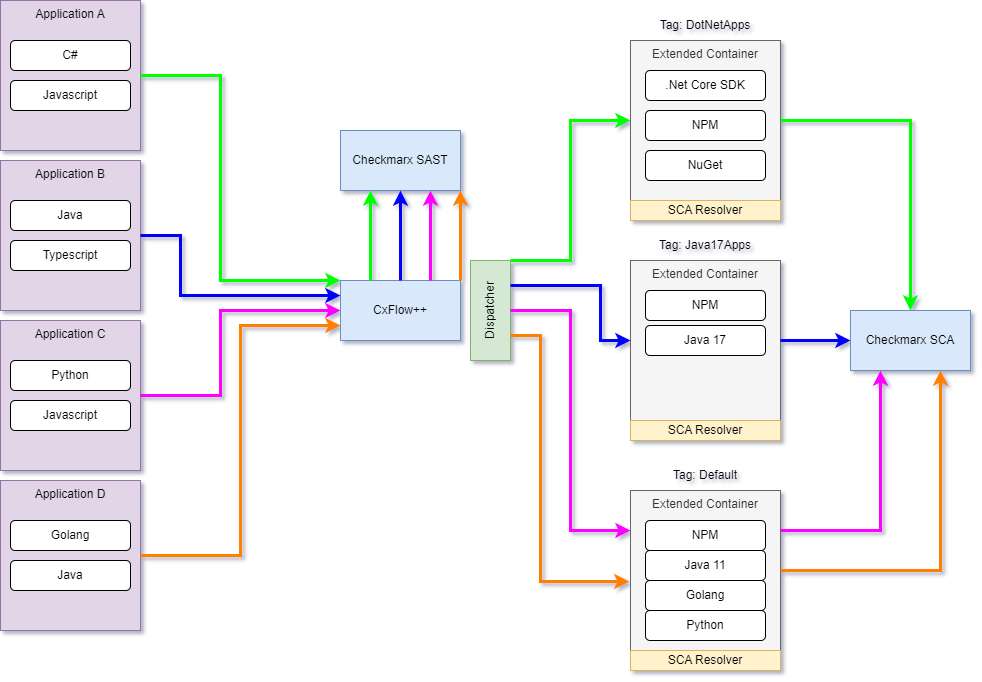
\includegraphics[width=\textwidth]{graphics/dispatcher_workflow.png}
    \label{fig:dispatcher_workflow}
\end{figure}


Some operational aspects of \cxflow may change when using \cxflowplusplus.  The \cxflowplusplus 
build environment affinity feature
\footnote{If there is no need to use this features of the dispatcher, \cxflowplusplus may not offer any advantages over \cxflow.} 
utilizes
\href{https://www.docker.com/blog/docker-can-now-run-within-docker/}{docker-in-docker (DIND)}; this may
change the compatibility of the runtime environment for an existing \cxflow deployment.

\subsection{\cxflowplusplus Runtime Environment}

The minimum recommended environment for \cxflowplusplus is:

\begin{itemize}
    \item 4 Cores
    \item 32 GB RAM
    \item 200GB of disk space
    \item Linux OS with kernel >= 5.12 if using \sysbox
\end{itemize}

\cxflowplusplus will be loading and executing container images as part of supply chain vulnerability scan
orchestration.  This can be potentially CPU and memory intensive.  Vertical or horizontal scaling
of \cxflowplusplus may be required to be able to orchestrate the volume of scans requested.

\noindent\\The execution of \cxflowplusplus must have some additional parameters provided to the
\texttt{docker} command to be able to create and execute docker containers inside the \cxflowplusplus
container.  If these additional parameters are not provided, \cxflowplusplus will emit errors when
attempting to execute docker containers inside the running container.

\subsubsection{DIND - Privileged Execution}

One method of enabling docker-in-docker is to execute containers in privileged mode.
Running \cxflowplusplus in privileged mode can be done like so:


\noindent\\\texttt{docker run -privileged -d ----restart unless-stopped \textbackslash }
\noindent\\ \tabto{5mm} \texttt{\cxflowplusplustag}

\noindent\\\textbf{WARNING}
\noindent\\It is generally considered a bad security practice to run a docker container in privileged mode.
Given that some open source packages can execute malware payloads during dependency resolution, it is not
advised to run in privileged mode for production purposes.

\subsubsection{DIND - \sysbox Runtime}

An alternative to executing docker in privileged mode is to use \sysbox as a runtime.  \sysbox runs on Linux
and has a requirement of a kernel version >= 5.12.  Appendix \ref{chap:sysbox_install} has
a procedure that can be used to install \sysbox manually on a Linux OS.

\noindent\\\texttt{docker run ----runtime=sysbox-runc -d ----restart unless-stopped \textbackslash}
\noindent\\ \tabto{5mm} \texttt{\cxflowplusplustag}

\subsection{Logging}

\cxflow logs to the console to maintain running compatibility with the official \cxflow image.  
Any supply chain vulnerability scan environment affinity operations are logged in files found
on the container in the directory \texttt{/var/log/dispatcher}.  To maintain the logs across
restarts of the container, it is recommended to map a local volume to \texttt{/var/log/dispatcher}.
The use of logging files for the dispatcher is to avoid the console logs from being corrupted
by spontaneous log emissions from the dispatcher.


\subsection{\cxflow Image Compatibility}

All the existing Spring Boot facilities for configuring \cxflow via environment variables work 
with the \cxflowplusplus image.  Using the \cxflowplusplus image in place of the official
\cxflow image is compatible as long as there is no need to execute \scaresolver.

If using \scaresolver, more configuration needed to provide a method of container image selection
for use in supply chain vulnerability scans.  The container will actively prevent
configuration of the \cxflow \texttt{SCA\_PATH\_TO\_SCA\_RESOLVER} option.  

The \cxflowplusplus image does not contain the \scaresolver runtime that would normally be found
in the official \cxflow image.  The \cxflowplusplus image replaces \scaresolver with
a mediation script known as \textit{the dispatcher} that invokes \scaresolver in an appropriate
container image.

The \cxflowplusplus image supports environment variables that change how it operates when 
preparing to start the \cxflow services.  Appendix \ref{chap:image_opts} has a complete list
of \cxflowplusplus additional options.


\subsection{Config-as-Code Build Environment Affinity}
When an supply chain vulnerability scan is invoked, the \texttt{default} 
image tag\footnote{The image tag refers to the tag of specified in the dispatcher configuration.  This should not be confused with the container tag.}
is used unless a config-as-code file is provided that explicitly defines the
image tag to use for the execution environment.

A config-as-code file named \texttt{.cxsca} should be placed in the root of the repository.  
The content of the file is JSON with the following structure:
\\
\begin{code}{.cxsca}{Config-as-Code Structure}{}
{
    "version" : "1",
    "tag" : "<dispatcher image tag>"
}
\end{code}

\subsection{\cxflowplusplus Dispatcher Configuration}

The dispatcher can configuration can be represented by either or both a YAML definition file and 
Environment variables.  The first YAML file found in \texttt{/dispatcher/yaml} when 
the dispatcher starts is used as the configuration file.  The configuration is 
evaluated in the following order of precedence:

\begin{enumerate}
\item Environment variables
\item YAML configuration
\end{enumerate}

\noindent\\This allows for environment variables to override YAML configurations or to provide
a combination of YAML and environment variable configured options.  A YAML configuration
file can be provided at runtime by mapping a local volume containing the configuration YAML to 
\texttt{/dispatcher/yaml}.  A YAML configuration file can alternately be provided at runtime
using the \hyperref[sec:DISPATCHERYAMLURL]{\texttt{DISPATCHER\_YAML\_URL}} \cxflowplusplus startup
environment variable. 

\noindent\\The complete reference for configuring the dispatcher can be found in
Appendix \ref{chap:dispatcher_config}.

